\documentclass[a4paper,12pt]{article}
\usepackage[spanish, es-tabla]{babel}
\usepackage[utf8]{inputenc}
\usepackage{url}
\usepackage{hyperref}  
\usepackage{amsmath}
\usepackage{graphicx}
\usepackage{multicol} 
\usepackage{float} 
\usepackage[left=2.00cm, right=2.00cm, top=2.00cm, bottom=2.00cm]{geometry} 
\author{Lidia del Moral Navarrete}
\title{Se trata del proyecto final del curso de Git y Latex, aunque la información esta sacada de recurso veraces los datos de tablas y demás son inventados}

\begin{document}

\begin{figure}[H]

\raggedright

\includegraphics[scale=0.4]{Darwin}\hfill
\includegraphics[scale=0.2]{IAS}

\end{figure}

\vspace{5mm}

\begin{center}
{\textbf{\Huge Aceites Vegetales}}
\vspace{2mm}

{\large Autor 1$^{1}$,Autor 2$^{1}$,Autor 3 $^{2}$}
\vspace{5mm}

$^{1}$ \textit{Universidad de Granada. Darwin Eventur.}

$^{2}$ \textit{Universidad de Córdoba. Instituto de Agricultura Sostenible.}

\end{center}

\vspace{3mm}

\begin{abstract}

\vspace{2mm}

URL del repositorio
 
\url{https://github.com/LdelMoral75/proyecto\_final}

\vspace{3mm}

En los últimos años, la producción y el consumo de aceites vegetales (palma, soja, colza, girasol, etc.) ha aumentado considerablemente, tanto para su uso en crudo como en procesos de cocinado; es el caso de la fritura.

Analizar el perfil de ácidos grasos de distintas fuentes vegetales (semillas) nos va a llevar a comprobar cuales son los aceites mas saludables, diferenciando los que podrán consumirse crudos, en frituras o aquellos que necesiten ser sometidos a refinación. 

Por cromatografía de gases (CG)  se obtendrá el perfil y porcentajes de los diferentes ácidos grasos que conforman los aceites.

La cromatografía de gases (CG) es una de las técnicas analíticas más empleadas para la determinación de compuestos orgánicos. La cromatografía de gases es una técnica sensible, que
requiere poca cantidad de muestra para el análisis (del orden de los µL) y que proporciona una alta resolución, siendo capaz de detectar concentraciones a niveles de ppm.
\vspace{2mm}

\textbf{Palabras clave:} \textit{Aceites vegetales, perfil de acidos grasos, cromatografía de gases, ppm.}


\end{abstract}
\vspace{3mm}

\begin{multicols}{2}
\section{Introducción}

Los aceites vegetales son líquidos naturales que se extraen de las plantas cuyos componentes mayoritarios son los triglicéridos, además de contener otros componentes minoritarios,como fenoles, alcoholes, tocoferoles y compuestos volátiles. Los ácidos grasos pueden ser saturados o insaturados, y su proporción en los aceites vegetales es lo que determina principalmente su estabilidad y propiedades, y lo que diferencia a los distintos aceites. Algunos pueden consumirse crudos (aceite de oliva virgen) mientras que otros solo se consumen tras ser sometidos a refinación (aceite de girasol)\cite{VELASCO1999}.

Mientras que las grasas vegetales presentan un alto contenido en ácidos grasos saturados y por lo tanto una consistencia sólida a temperatura ambiente, los aceites de semillas por poseer multitud de ácidos grasos monoinsaturados y poliinsaturados, tienen consistencia líquida a temperatura ambiente.

Los estudios muestran que comer alimentos ricos en grasas insaturadas en lugar de grasas saturadas mejora los niveles de colesterol en la sangre, lo que puede disminuir el riesgo de ataque cardíaco y de accidente cerebrovascular \cite{Andarwulan2014}.

Sin embargo, las grasas con un elevado contenido en ácidos grasos saturados son las mejores para los procesos de fritura, pero su efecto sobre la salud es muy perjudicial ya que elevan el colesterol LDL (malo). Un colesterol LDL alto incrementa su riesgo de enfermedad cardíaca y accidente cerebrovascular.

Cuando se fríe o cocina a altas temperaturas (a unos 180C) se produce un cambio en las estructuras moleculares de los aceites y grasas que se utilizan \cite{Burton2022}.

Pasan por un proceso que se llama oxidación, por el cual reaccionan con el oxígeno en el aire para formar aldehídos y peróxidos lípidos, perjudiciales para la salud.

Los aceites ricos en acidos grasos poliinsaturados,como el aceite de maíz o el aceite de girasol, generan niveles muy altos de aldehídos.Sin embargo, el aceite de oliva y el de colza generaron muchos menos aldehídos, igual que la mantequilla y la grasa de ganso.

El motivo es que estos aceites son más ricos en ácidos grasos saturados y monoinsaturados, y estos son mucho más estables cuando se calientan.

De hecho, las grasas saturadas apenas pasan por esa reacción de oxidación.

Por lo tanto, debemos diferenciar el uso de los aceites según vayan a ser consumidos crudos o en fritura.

\section{Metodología}

La investigación se ha llevado a cabo a partir de 12 muestras de diferentes aceites: coco, palma , oliva, cacahuete, colza, algodón, ricino, maíz, girasol, soja, cártamo y lino de las que se va a determinar la composición de ácidos grasos.

Por cromatografía de gases se va a determinar la composición en ácidos grasos de estos aceites. Este proceso consta de dos partes: 
\begin{itemize}
\item Preparación de esteres metílicos de ácidos grasos.

\item Análisis por cromatografía de gases de los esteres metílicos de ácidos grasos.
\end{itemize}

Debido a que los ácidos grasos tienen baja volatilidad para poder analizarlos por cromatografía de gases es necesario transformarlos en sus ésteres metílicos. Los ésteres metílicos se forman por la transesterificacion del aceite vegetal con una disolución metanólica de hidróxido de potasio como una fase intermedia antes de que se produzca la saponificación siguiendo el punto 5 del método ISO 5509-2000.
\begin{itemize}

\item Preparación de los ésteres metílicos:

Los reactivos que vamos a utilizar son: metanol, heptano para cromatografía, hidróxido potásico.

En un tubo roscado se pesan 0,1 gramo de la muestra de aceite, añadimos 2ml de heptano y agitamos, sobre ello 0,2 ml de solución metanólica de hidróxido potásico, tapamos  y agitamos 30 segundos aproximadamente. Dejamos reposar hasta que la capa superior de la disolución este nítida. Analizaremos esta capa superior que es la que contiene los esteres metílicos.

\item Análisis por cromatografía de gases de los ésteres metílicos:

La cromatografía de gases es la técnica más empleada y aceptada para la determinación de ácidos grasos \cite{VELASCO1999,Sineiro1998}.

El cromatógrafo de gases consta principalmente de un inyector para introducir la muestra en el sistema, una columna en la que se separan los distintos componentes de la muestra según
su afinidad por la fase estacionaria, un horno para suministrar calor a la columna y un detector que proporciona la señal analítica.

El programa de temperatura utilizado es comenzamos a 150 grados centígrados de temperatura y vamos aumentando la temperatura 5 grados por minuto hasta alcanzar los 240 grados centígrados, a esa temperatura dejaremos los gases durante 10 minutos (Figura 1).
\begin{figure}[H]

\raggedright
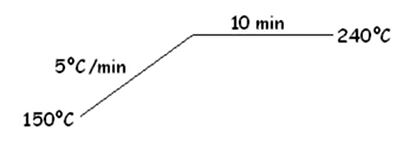
\includegraphics[scale=0.9]{Temperaturahorno}
\caption{Programa de temperaturas}
\label{fig: Figura 1}
\end{figure}

Después procederemos a pinchar la muestra, los esteres de ácidos grasos que se han preparado. El volumen de inyección sera de 1 microlitro. El cromatograma correspondiente a la muestra aparecerá en el monitor.

Cada soluto contenido en la mezcla se mueve con su propia velocidad según sus propiedades físicas y químicas (peso molecular, punto de ebullición, polaridad). 
El tiempo de aparición $(t^r)$ de cada pico identifica a cada componente de la mezcla, y el área $(W)$ indica la fracción presente del mismo.

\begin{equation*}
\% Acidos grasos = (t^r / W)^2 
\end{equation*}
\textit{(Formula totalmente inventada para este proyecto LaTex)}
\end{itemize}

\section{Resultados y discusión}

Los ácidos grasos saturados, aquellos que no poseen dobles enlaces, como el ácido mirístico, palmítico, esteárico y láurico los podemos encontrar en una gran cantidad en las grasas de origen animal y en algunos aceites de origen vegetal(coco y palma)muy usados para elaborar alimentos de repostería industrial, snacks de aperitivo, etc. Además, tratamientos industriales como la hidrogenación, que se aplica en algunos aceites vegetales, aumentan la porción de estos ácidos grasos saturados.

Los ácidos grasos saturados son muy estables. En términos de utilización, esto significa que pueden soportar elevadas temperaturas y almacenarse durante largos períodos, a la vez que a temperatura ambiente se vuelven sólidos.

De los ácidos grasos monoinsaturados, con un solo doble enlace en su cadena, el ácido oleico es el más abundante y se encuentra presente principalmente en alimentos de origen vegetal, sobre todo en el aceite de oliva, a diferencia del ácido palmitoleico cuya presencia es poco común en la grasa vegetal.

Se recomienda su ingesta ya que disminuyen considerablemente los niveles de colesterol-LDL (lipoproteína de baja densidad) asociado a enfermedades cardiovasculares, sin modificar el colesterol-HDL (lipoproteína de alta densidad)\cite{Andarwulan2014,Orsavova2015}. 

Los ácidos grasos poliinsaturada, con mas de un doble enlace en su cadena, también se encuentra en aceites vegetales especialmente en el de girasol, maíz y soja, así como en las nueces y otros frutos secos y en el pescado azul. Dentro de este grupo se encuentran el ácido linoleico (omega-6) y linolénico (omega-3) denominados “ácidos grasos esenciales” ya que no pueden ser sintetizados por el organismo, y por lo tanto solo pueden obtenerse a través de la dieta. Un buen equilibrio entre ambos reduce el riesgo de enfermedad cardiovascular y ademas son necesarios para la generación de células \cite{NasiffHadad2003,AlfonsoValenzuela}.

Los ácidos grasos trans son formas de ácidos grasos insaturados con una cadena lineal en lugar de una cadena doblada. Se forman como subproductos de la hidrogenación de aceites. No pueden ser metabolizados en el organismo de la misma manera y su consumo crónico ha sido ligado a varias afecciones, por lo que su contenido está regulado por normas \cite{BarreraArellano1993}.

Se encuentra en aceites baratos utilizados para la fritura, alimentos precocinados, pizzas congeladas, algunas mantecas vegetales, bollería y pastelería industrial, galletas saladas y dulces industriales, helados, cremas de café, glaseados listos para usar, patatas fritas “de bolsa”, aperitivos, chucherías y palomitas de microondas. Su objetivo es conservar la duración de los alimentos, mejorar su sabor o favorecer la estabilidad en la fritura. 

Por su relación con la incidencia de enfermedades cardiovasculares, el estudio del perfil de los ácidos grasos en los aceites vegetales es de gran importancia \cite{Ucciani1994}. 

Ademas, es importante recordar que las grasas insaturadas, al tener mayor número de insaturaciones, son más inestables y susceptibles a la oxidación que las monoinsaturadas, lo que puede dar lugar a la aparición de sustancias tóxicas cuando se someten a altas temperaturas durante el cocinado, por ejemplo en las frituras. Por este motivo es importante utilizar aceite de oliva no solo en crudo sino también para cocinar ya que es mucho más estable y aguanta mejor las altas temperaturas \cite{Balaciano}.

El resultado del análisis por cromatografía de gases de los  ácidos grasos de las 12 muestras de las que partíamos se muestra a continuación en la siguiente tabla (Tabla 1)(Figura 2).

\end{multicols}

\begin{table}[H]
\centering
\begin{tabular}{|c|c|c|}
\hline

Aceite & Principal Ácido Graso & \% Ácido Graso Principal\\
\hline
Coco & Láurico C12:0 & 44-52\\
\hline
Palma & Palmítico C16:0 & 30-40\\
\hline
Oliva & Oleico C18:1 & 70-86\\
\hline
Cacahuete & Oleico C18:1 & 40-70\\
\hline
Colza & Erúcico C22:1 & 48-60\\
\hline
Algodón & Linoleico C18:2 & 40-55\\
\hline
Ricino & Ricinoleico C18:1 & 80-90\\
\hline
Maiz & Oleico, linoleico C18:2 & 34-62\\
\hline
Girasol & Linoleico C18:2 & 48-74\\
\hline
Soja & Linoleico C18:2 & 52-60\\
\hline
Cártamo & Linoleico C18:2 & 78\\
\hline
Lino & Linoleico C18:2 & 30-60\\
\hline

\end{tabular}
\caption{Tabla de Ácidos grasos}
\label{tb: Tabla 1}
\end{table}

\begin{figure}[H]
\centering
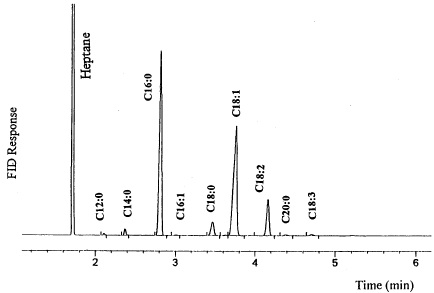
\includegraphics[scale=0.9]{cromatograma}
\caption{Cromatograma}
\label{fig: Figura 2}
\end{figure}

\vspace{3mm}

\begin{multicols}{2}

Los aceites vegetales son ampliamente comercializados
en el mercado internacional. Siendo los aceites de palma,
soya, colza y girasol son los de mayor participación
en el mercado mundial.

\textit{Aceite de oliva}

Sin duda el aceite de oliva virgen extra es uno de los grandes patrimonios alimentarios de la humanidad, pero no es el único aceite vegetal que existe. Es el mejor para cocinar y freir, porque sus grasa monoinsaturadas son mas resistentes a la temperatura que los aceites poliinsaturados \cite{Berdeaux2012, Leon2018}.

En cada región del mundo se utiliza para cocinar aquel que más abunda en el entorno. De este modo, el aceite más usado en el continente americano es el de soja, pero en el sudeste asiático se utiliza sobre todo los aceites de sésamo, coco y cacahuete. Siendo en  África habitual el aceite de palma.

Otros aceites, minoritarios y presentes solo en determinadas gastronomías locales, también destacan por sus propiedades medicinales y sus aportes nutricionales, como es el caso de los aceites de nuez o linaza. 


\textit{Aceite de linaza}

Se extrae de la semilla del lino, conocida como linaza. Formado mayoritariamente por ácidos grasos insaturados, predominando entre un 20 y un 27\% de ácido oleico, y sobre todo entre un 53 y 57\% de ácido alfa-linolénico, que forma parte de los ácidos grasos Omega-3 y es esencial para el ser humano.

Adicionalmente puede tener también hasta un 22\% de ácido linoleico, otro ácido esencial. Dada su riqueza en ácidos esenciales, se puede usar en dietas veganas como complemento, ya sea ingiriendo una cucharada o bien de acompañamiento en ensaladas. No siendo apto para freír.

\textit{Aceite de canola}

El aceite de colza o canola se extrae de la semilla de la colza y se emplea como condimento en el norte de Europa, siendo Alemania su principal consumidor, donde prácticamente se usa en exclusiva. 

Es muy rico en un ácido graso monoinsaturado conocido como ácido erúcico, al cual se relaciona con posibles problemas cardiovasculares, aunque a grandes dosis. Además es rico en ácidos grasos esenciales: alfa-linolénico y linoleico.

\textit{Aceite de coco}

El aceite de coco es especialmente celebrado en muchos países por su sabor dulce característico y su estructura mantecosa y semisólida, ya que contiene un alto porcentaje de ácidos grasos saturados y muy pocos insaturados (apenas un 8\%). Se utiliza en la cocina de sudeste asiático como condimento, base de sopas o salsa para preparar curris, carnes y pescados, así como también en muchos platos africanos. Debido a su estructura, también se usa como grasa hidrogenada.

\textit{Aceite de girasol}

El aceite de girasol es el más usado en nuestro país, así como también en Francia, tras el de oliva. Posee una elevada proporción de ácido linoleico (esencial) y vitamina E. No es bueno para freír, al menos no tanto como el aceite de oliva, pero sí para ensaladas o mayonesas dado su toque suave \cite{FernandezMartinez2009}. 

\textit{Aceite de soja}

Es el aceite de mayor producción mundial, por delante del de girasol y el de colza. Nutricionalmente destaca por su riqueza en ácido alfa- linolénico, si bien tiene mayor proporción de ácidos grasos poliinsaturados frente a los monoinsaturados. 

\textit{Aceite de maíz}

Es otro aceite de amplio uso por su precio asequible y por tener una baja propoción de grasa saturadas, aunque en su composición dominan las poliinsaturadas. Se utiliza erróneamente con asiduidad para freír cuando por su sabor poco pronunciado es ideal para ensaladas, salsas o mayonesas.

\textit{Aceite de palma}

El aceite de palma es el más utilizado del mundo, por delante del de soja o el de colza. Se produce a partir de los frutos de la palma africana (Elaeis guineensis) y se ha convertido en una materia prima usada a nivel global para la elaboración de una gran cantidad de productos de la industria alimentaria y cosmética.
 
El aceite de palma está desplazando a las grasas hidrogenadas, que se han demostrado nocivas para la salud. No obstante, este aceite es muy rico en grasas saturadas, por lo que está lejos de ser una alternativa idónea desde el punto de vista del equilibrio nutricional y es preferible no abusar de él.

\textit{Aceite de cacahuete}

Se obtiene del prensado del cacahuete y tiene una buena proporción de ácidos grasos monoinsaurados, sobre todo oleico, que puede llegar a ser el 72\%, y poliinsaturados, principalmente linoleico. Aguanta bien las altas temperaturas, por lo que en Asia se lo usa con frecuencia para las preparaciones en wok. Por su sabor suave y neutro, es adecuado para vinagretas, mayonesas y ensaladas.

\textit{Aceite de cártamo}

Se extrae de la semilla de la planta de cártamo. Posee una alta cantidad de grasas poliinsaturadas (ácido linoleico) y es adecuado usarlo para ensaladas y como aceite de cocina. El aceite de cártamo que posee un nivel muy alto de grasa monoinsaturada (ácido oleico) está disponible para la industria alimentaria para su uso como aceite para freír \cite{Hamdan2009a,Hamdan2009}.



\section{Bibliografía}

\bibliography{Bibliografiaproyecto}
\bibliographystyle{plain}


\end{multicols}

\end{document}
















